% Tín hiệu số với dãy bit 0 1 0 0 1 0 1 1, vẽ lại từ hình mẫu.
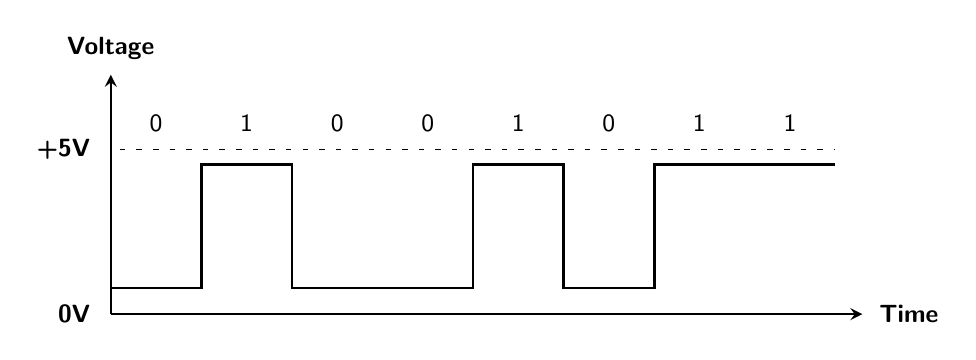
\begin{tikzpicture}[x=1.15cm, y=0.95cm, font=\sffamily\small]
    % Trục điện áp và thời gian.
    \draw[->, >=stealth, line width=0.9pt] (0, 0) -- (0, 3.2);
    \draw[->, >=stealth, line width=0.9pt] (0, 0) -- (8.3, 0);
    \node[anchor=south, font=\sffamily\small\bfseries]
        at (0, 3.28) {Voltage};
    \node[anchor=west, font=\sffamily\small\bfseries]
        at (8.38, 0) {Time};

    % Mức điện áp tham chiếu, giữ cách trình bày của hình mẫu.
    \draw[dash pattern=on 2pt off 4pt, line width=0.6pt]
        (0.1, 2.2) -- (8, 2.2);
    \node[anchor=east, font=\sffamily\small\bfseries]
        at (-0.12, 2.2) {+5V};
    \node[anchor=east, font=\sffamily\small\bfseries]
        at (-0.12, 0) {0V};

    % Các khoảng bit có độ dài bằng nhau.
    \foreach \position/\bit in {0.5/0, 1.5/1, 2.5/0, 3.5/0,
                                4.5/1, 5.5/0, 6.5/1, 7.5/1} {
        \node at (\position, 2.55) {\bit};
    }

    % Xung vuông: các bit liên tiếp cùng giá trị giữ nguyên mức.
    \draw[line width=1pt, line join=miter, line cap=butt]
        (0, 0.35) -- (1, 0.35)
        -- (1, 2) -- (2, 2)
        -- (2, 0.35) -- (4, 0.35)
        -- (4, 2) -- (5, 2)
        -- (5, 0.35) -- (6, 0.35)
        -- (6, 2) -- (8, 2);
\end{tikzpicture}
